\documentclass[]{book}
\usepackage{lmodern}
\usepackage{amssymb,amsmath}
\usepackage{ifxetex,ifluatex}
\usepackage{fixltx2e} % provides \textsubscript
\ifnum 0\ifxetex 1\fi\ifluatex 1\fi=0 % if pdftex
  \usepackage[T1]{fontenc}
  \usepackage[utf8]{inputenc}
\else % if luatex or xelatex
  \ifxetex
    \usepackage{mathspec}
  \else
    \usepackage{fontspec}
  \fi
  \defaultfontfeatures{Ligatures=TeX,Scale=MatchLowercase}
\fi
% use upquote if available, for straight quotes in verbatim environments
\IfFileExists{upquote.sty}{\usepackage{upquote}}{}
% use microtype if available
\IfFileExists{microtype.sty}{%
\usepackage{microtype}
\UseMicrotypeSet[protrusion]{basicmath} % disable protrusion for tt fonts
}{}
\usepackage[margin=1in]{geometry}
\usepackage{hyperref}
\hypersetup{unicode=true,
            pdftitle={Notes on Various Topics},
            pdfauthor={서용덕 Yongduek Seo yndk@sogang.ac.kr},
            pdfborder={0 0 0},
            breaklinks=true}
\urlstyle{same}  % don't use monospace font for urls
\usepackage{natbib}
\bibliographystyle{apalike}
\usepackage{color}
\usepackage{fancyvrb}
\newcommand{\VerbBar}{|}
\newcommand{\VERB}{\Verb[commandchars=\\\{\}]}
\DefineVerbatimEnvironment{Highlighting}{Verbatim}{commandchars=\\\{\}}
% Add ',fontsize=\small' for more characters per line
\usepackage{framed}
\definecolor{shadecolor}{RGB}{248,248,248}
\newenvironment{Shaded}{\begin{snugshade}}{\end{snugshade}}
\newcommand{\KeywordTok}[1]{\textcolor[rgb]{0.13,0.29,0.53}{\textbf{#1}}}
\newcommand{\DataTypeTok}[1]{\textcolor[rgb]{0.13,0.29,0.53}{#1}}
\newcommand{\DecValTok}[1]{\textcolor[rgb]{0.00,0.00,0.81}{#1}}
\newcommand{\BaseNTok}[1]{\textcolor[rgb]{0.00,0.00,0.81}{#1}}
\newcommand{\FloatTok}[1]{\textcolor[rgb]{0.00,0.00,0.81}{#1}}
\newcommand{\ConstantTok}[1]{\textcolor[rgb]{0.00,0.00,0.00}{#1}}
\newcommand{\CharTok}[1]{\textcolor[rgb]{0.31,0.60,0.02}{#1}}
\newcommand{\SpecialCharTok}[1]{\textcolor[rgb]{0.00,0.00,0.00}{#1}}
\newcommand{\StringTok}[1]{\textcolor[rgb]{0.31,0.60,0.02}{#1}}
\newcommand{\VerbatimStringTok}[1]{\textcolor[rgb]{0.31,0.60,0.02}{#1}}
\newcommand{\SpecialStringTok}[1]{\textcolor[rgb]{0.31,0.60,0.02}{#1}}
\newcommand{\ImportTok}[1]{#1}
\newcommand{\CommentTok}[1]{\textcolor[rgb]{0.56,0.35,0.01}{\textit{#1}}}
\newcommand{\DocumentationTok}[1]{\textcolor[rgb]{0.56,0.35,0.01}{\textbf{\textit{#1}}}}
\newcommand{\AnnotationTok}[1]{\textcolor[rgb]{0.56,0.35,0.01}{\textbf{\textit{#1}}}}
\newcommand{\CommentVarTok}[1]{\textcolor[rgb]{0.56,0.35,0.01}{\textbf{\textit{#1}}}}
\newcommand{\OtherTok}[1]{\textcolor[rgb]{0.56,0.35,0.01}{#1}}
\newcommand{\FunctionTok}[1]{\textcolor[rgb]{0.00,0.00,0.00}{#1}}
\newcommand{\VariableTok}[1]{\textcolor[rgb]{0.00,0.00,0.00}{#1}}
\newcommand{\ControlFlowTok}[1]{\textcolor[rgb]{0.13,0.29,0.53}{\textbf{#1}}}
\newcommand{\OperatorTok}[1]{\textcolor[rgb]{0.81,0.36,0.00}{\textbf{#1}}}
\newcommand{\BuiltInTok}[1]{#1}
\newcommand{\ExtensionTok}[1]{#1}
\newcommand{\PreprocessorTok}[1]{\textcolor[rgb]{0.56,0.35,0.01}{\textit{#1}}}
\newcommand{\AttributeTok}[1]{\textcolor[rgb]{0.77,0.63,0.00}{#1}}
\newcommand{\RegionMarkerTok}[1]{#1}
\newcommand{\InformationTok}[1]{\textcolor[rgb]{0.56,0.35,0.01}{\textbf{\textit{#1}}}}
\newcommand{\WarningTok}[1]{\textcolor[rgb]{0.56,0.35,0.01}{\textbf{\textit{#1}}}}
\newcommand{\AlertTok}[1]{\textcolor[rgb]{0.94,0.16,0.16}{#1}}
\newcommand{\ErrorTok}[1]{\textcolor[rgb]{0.64,0.00,0.00}{\textbf{#1}}}
\newcommand{\NormalTok}[1]{#1}
\usepackage{longtable,booktabs}
\usepackage{graphicx,grffile}
\makeatletter
\def\maxwidth{\ifdim\Gin@nat@width>\linewidth\linewidth\else\Gin@nat@width\fi}
\def\maxheight{\ifdim\Gin@nat@height>\textheight\textheight\else\Gin@nat@height\fi}
\makeatother
% Scale images if necessary, so that they will not overflow the page
% margins by default, and it is still possible to overwrite the defaults
% using explicit options in \includegraphics[width, height, ...]{}
\setkeys{Gin}{width=\maxwidth,height=\maxheight,keepaspectratio}
\IfFileExists{parskip.sty}{%
\usepackage{parskip}
}{% else
\setlength{\parindent}{0pt}
\setlength{\parskip}{6pt plus 2pt minus 1pt}
}
\setlength{\emergencystretch}{3em}  % prevent overfull lines
\providecommand{\tightlist}{%
  \setlength{\itemsep}{0pt}\setlength{\parskip}{0pt}}
\setcounter{secnumdepth}{5}
% Redefines (sub)paragraphs to behave more like sections
\ifx\paragraph\undefined\else
\let\oldparagraph\paragraph
\renewcommand{\paragraph}[1]{\oldparagraph{#1}\mbox{}}
\fi
\ifx\subparagraph\undefined\else
\let\oldsubparagraph\subparagraph
\renewcommand{\subparagraph}[1]{\oldsubparagraph{#1}\mbox{}}
\fi

%%% Use protect on footnotes to avoid problems with footnotes in titles
\let\rmarkdownfootnote\footnote%
\def\footnote{\protect\rmarkdownfootnote}

%%% Change title format to be more compact
\usepackage{titling}

% Create subtitle command for use in maketitle
\newcommand{\subtitle}[1]{
  \posttitle{
    \begin{center}\large#1\end{center}
    }
}

\setlength{\droptitle}{-2em}

  \title{Notes on Various Topics}
    \pretitle{\vspace{\droptitle}\centering\huge}
  \posttitle{\par}
    \author{서용덕 Yongduek Seo
\href{mailto:yndk@sogang.ac.kr}{\nolinkurl{yndk@sogang.ac.kr}}}
    \preauthor{\centering\large\emph}
  \postauthor{\par}
      \predate{\centering\large\emph}
  \postdate{\par}
    \date{2018-09-30}

\usepackage{booktabs}
\usepackage{kotex}

\usepackage{amsthm}
\newtheorem{theorem}{Theorem}[chapter]
\newtheorem{lemma}{Lemma}[chapter]
\theoremstyle{definition}
\newtheorem{definition}{Definition}[chapter]
\newtheorem{corollary}{Corollary}[chapter]
\newtheorem{proposition}{Proposition}[chapter]
\theoremstyle{definition}
\newtheorem{example}{Example}[chapter]
\theoremstyle{definition}
\newtheorem{exercise}{Exercise}[chapter]
\theoremstyle{remark}
\newtheorem*{remark}{Remark}
\newtheorem*{solution}{Solution}
\begin{document}
\maketitle

{
\setcounter{tocdepth}{1}
\tableofcontents
}
\chapter{Prerequisites}\label{prerequisites}

Read linear algebra, probability and statistics, computer programming to
do data science.

\chapter{Gradient Boosting}\label{gradient-boosting}

\section{Useful links to read}\label{useful-links-to-read}

\begin{enumerate}
\def\labelenumi{\arabic{enumi}.}
\item
  \href{https://medium.com/mlreview/gradient-boosting-from-scratch-1e317ae4587d}{Gradient
  Boosting from scratch}
\item
  \href{http://explained.ai/gradient-boosting/index.html}{How to explain
  gradient boosting by Terence Parr and Jeremy Howard}
\item
  \href{https://quantdare.com/what-is-the-difference-between-bagging-and-boosting/}{What
  is the difference between Bagging and Boosting}
\item
  \href{https://www.ncbi.nlm.nih.gov/pmc/articles/PMC3885826/}{Gradient
  boosting machines (GBM), A Tutorial}
\item
  Use \href{https://xgboost.ai/}{XGBoost}.
\end{enumerate}

\section{Gradient Boosting from
Scratch}\label{gradient-boosting-from-scratch}

The reason we use ensembles is that many different predictors trying to
predict same target variable will perform a better job than any single
predictor alone.

\begin{figure}

{\centering 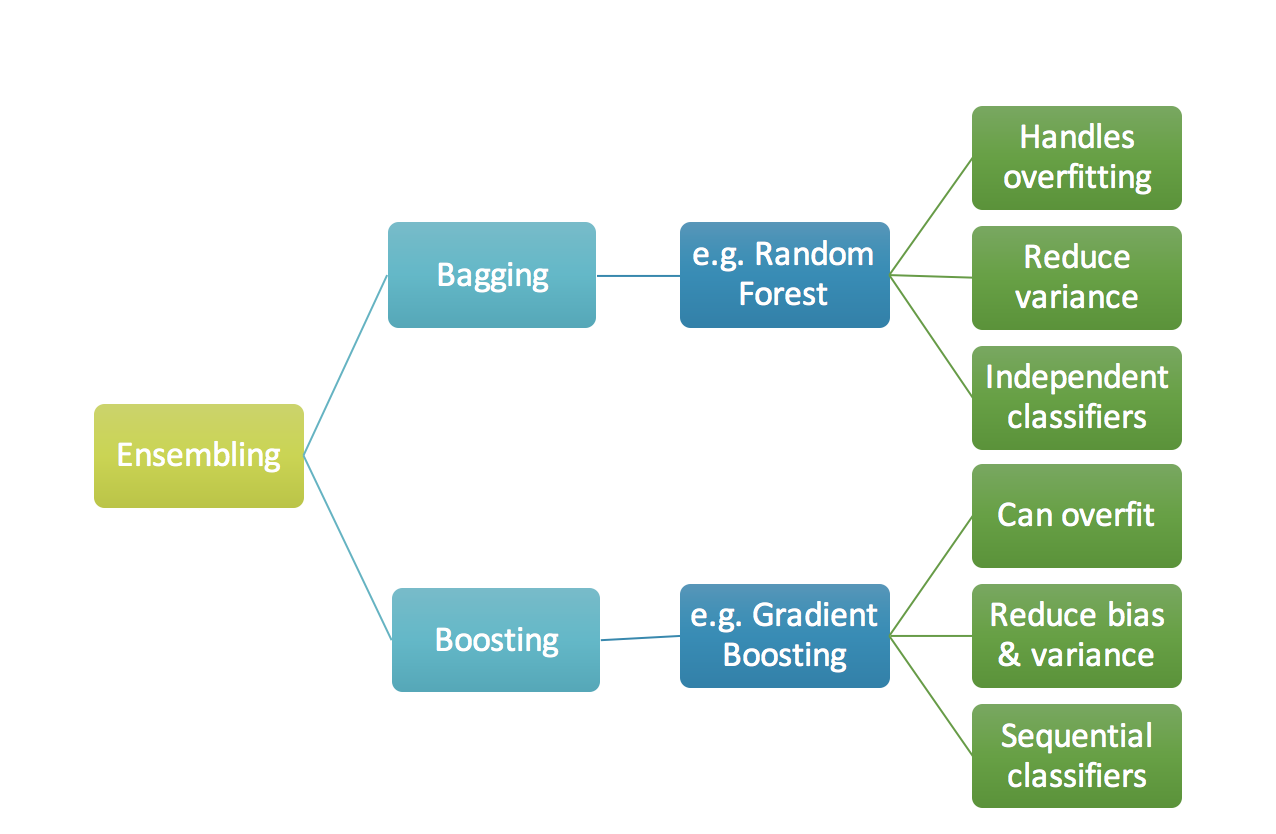
\includegraphics[width=0.7\linewidth]{figures/ensembling} 

}

\caption{Two branches of ensemble-based learning}\label{fig:ensembling}
\end{figure}

Ensembling techniques are further classified into Bagging and Boosting.

\begin{enumerate}
\def\labelenumi{\arabic{enumi}.}
\item
  \textbf{Bagging} is a simple ensembling technique in which we build
  many independent predictors/models/learners and combine them using
  some model averaging techniques. (e.g.~weighted average, majority vote
  or normal average). We typically take random sub-sample/bootstrap of
  data for each model, so that all the models are little different from
  each other. Each observation is chosen with replacement to be used as
  input for each of the model. So, each model will have different
  observations based on the bootstrap process. Because this technique
  takes many uncorrelated learners to make a final model, it reduces
  error by reducing variance. Example of bagging ensemble is Random
  Forest models.
\item
  \textbf{Boosting} is an ensemble technique in which the predictors are
  not made independently, but sequentially. This technique employs the
  logic in which the subsequent predictors learn from the mistakes of
  the previous predictors. Therefore, the observations have an unequal
  probability of appearing in subsequent models and ones with the
  highest error appear most. (So the observations are not chosen based
  on the bootstrap process, but based on the error). The predictors can
  be chosen from a range of models like decision trees, regressors,
  classifiers etc. Because new predictors are learning from mistakes
  committed by previous predictors, it takes less time/iterations to
  reach close to actual predictions. But we have to choose the stopping
  criteria carefully or it could lead to overfitting on training data.
  Gradient Boosting is an example of boosting algorithm.
\end{enumerate}

\begin{figure}

{\centering 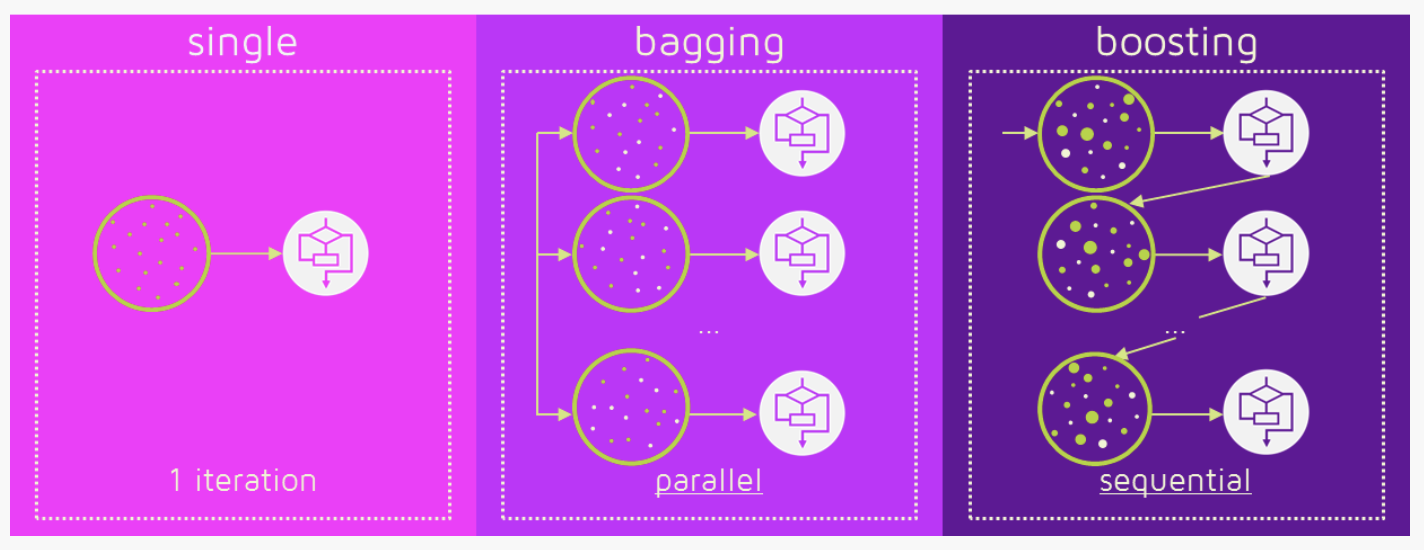
\includegraphics[width=0.8\linewidth]{figures/bagging-boosting} 

}

\caption{Bagging (independent models), Boosting (sequential models)}\label{fig:bagging-boosting}
\end{figure}

\section{\texorpdfstring{\href{http://explained.ai/gradient-boosting/index.html}{How
to explain gradient boosting by Terence Parr and Jeremy
Howard}}{How to explain gradient boosting by Terence Parr and Jeremy Howard}}\label{how-to-explain-gradient-boosting-by-terence-parr-and-jeremy-howard}

Gradient boosting machines (GBMs) are currently very popular and so it's
a good idea for machine learning practitioners to understand how GBMs
work. The problem is that understanding all of the mathematical
machinery is tricky and, unfortunately, these details are needed to tune
the hyper-parameters. (Tuning the hyper-parameters is required to get a
decent GBM model unlike, say, Random Forests.) Our goal in this article
is to explain the intuition behind gradient boosting, provide
visualizations for model construction, explain the mathematics as simply
as possible, and answer thorny questions such as why GBM is performing
``gradient descent in function space.''

\begin{figure}

{\centering 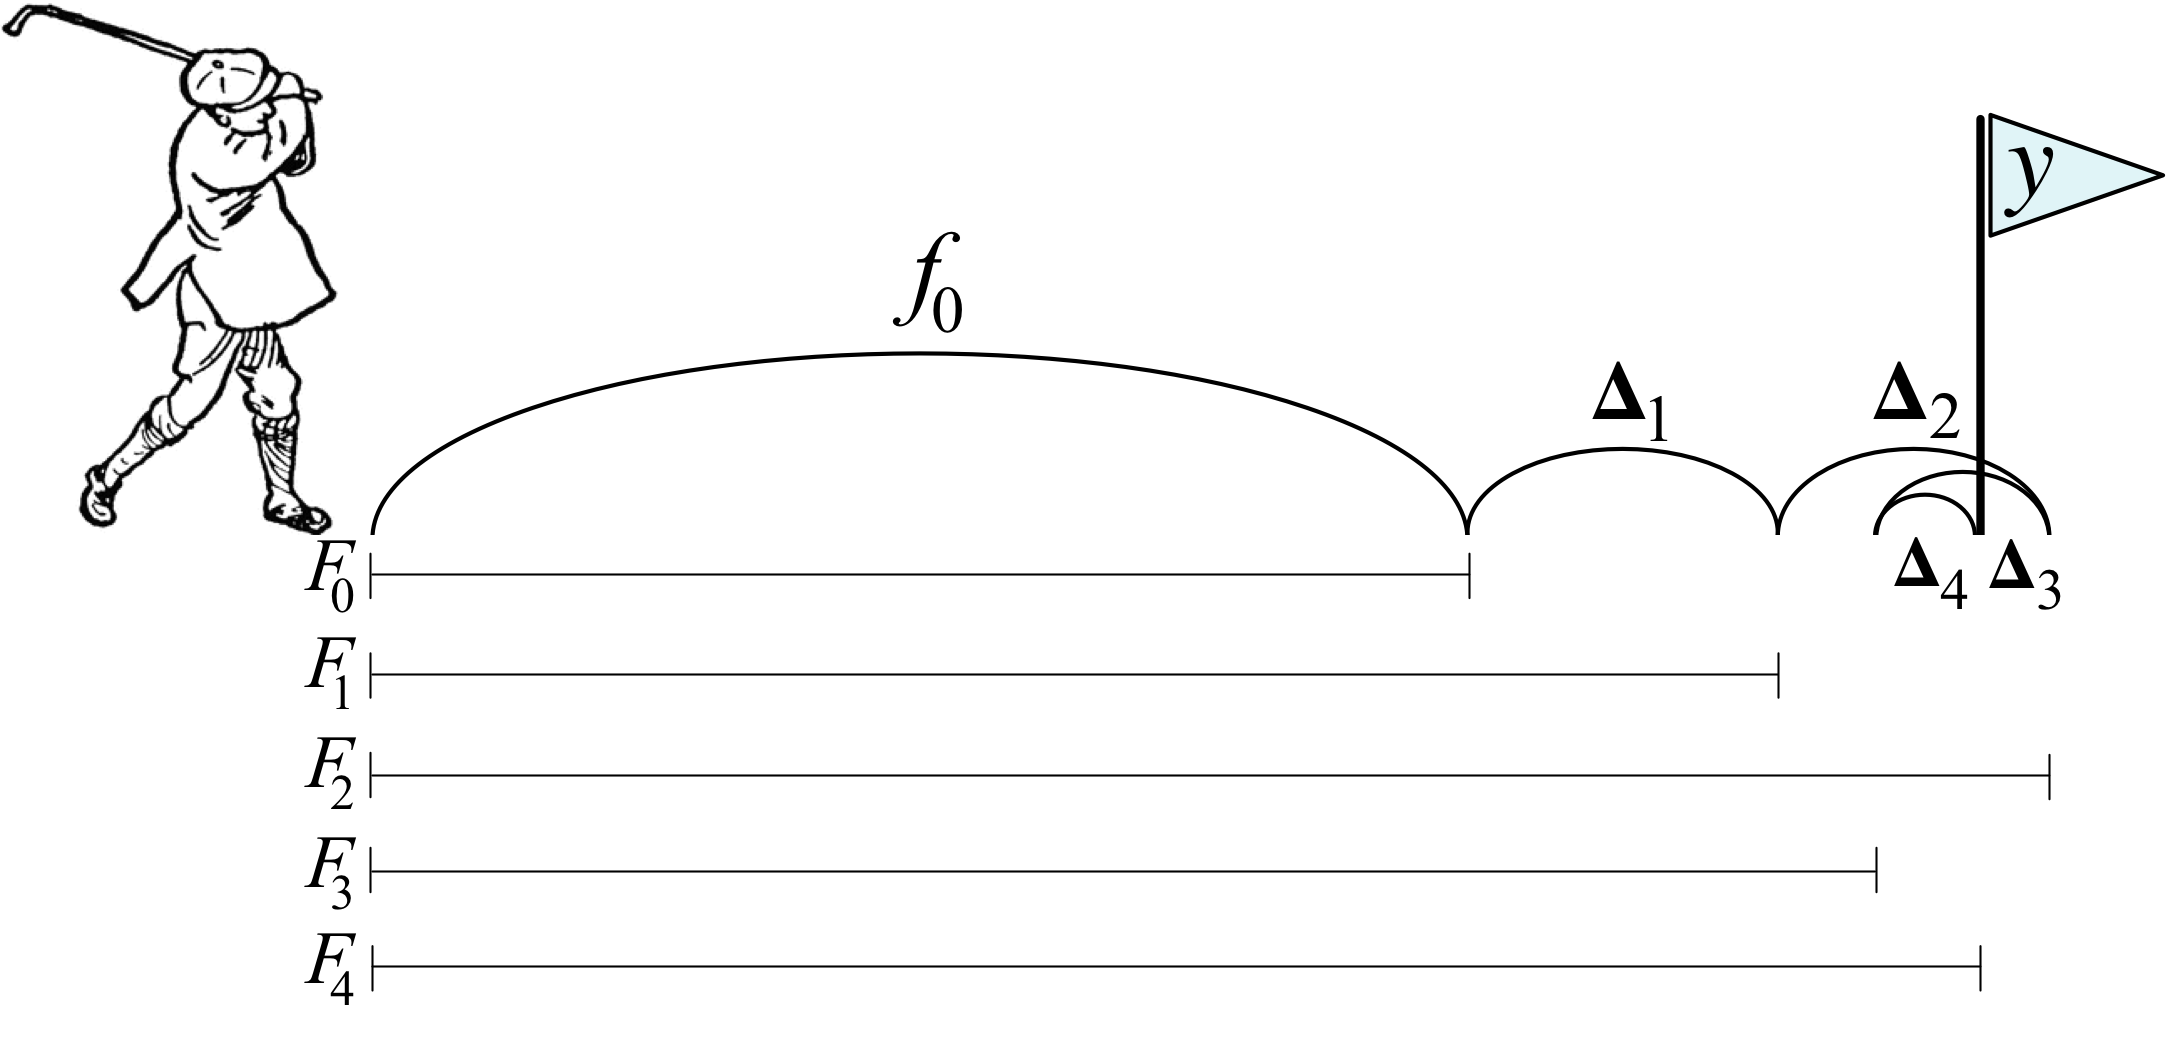
\includegraphics[width=0.8\linewidth]{figures/golf-dir-vector} 

}

\caption{Bagging (independent models), Boosting (sequential models)}\label{fig:golf-dir-vector}
\end{figure}

\subsection{The intuition behind gradient
boosting}\label{the-intuition-behind-gradient-boosting}

To construct a boosted regression model, let's start by creating a
crappy model, , that predicts an initial approximation of y given
feature vector . Then, let's gradually nudge the overall model towards
the known target value y by adding one or more tweaks, :

\begin{eqnarray*}
\hat y & = & f_0(\vec x) + \Delta_1(\vec x) + \Delta_2(\vec x) + ...  +  \Delta_M(\vec x) \\
 & = & f_0(\vec x) + \sum_{m=1}^M  \Delta_m(\vec x)\\
 & = & F_M(\vec x)\\
\end{eqnarray*}

Or, using a recurrence relation, let:

\begin{eqnarray*}
F_0(\vec x) &=& f_0(\vec x)\\
F_m(\vec x) &=& F_{m-1}(\vec x) + \Delta_m(\vec x)\\
\end{eqnarray*}

A sequential construction of a regression tree stump (depth 1 tree) is
the main procedure of the algorithm of gradient boosting machine.

Keep reading in
\href{http://explained.ai/gradient-boosting/L2-loss.html}{explained.ai},
which explains best.

\subsection{Gradient boosting regression by
example}\label{gradient-boosting-regression-by-example}

Imagine that we have square footage data on five apartments and their
rent prices in dollars per month as our training data:

\begin{table}

\caption{\label{tab:unnamed-chunk-2}data table}
\centering
\begin{tabular}[t]{r|r}
\hline
sqfeet & rent\\
\hline
750 & 1160\\
\hline
800 & 1200\\
\hline
850 & 1280\\
\hline
900 & 1450\\
\hline
950 & 2000\\
\hline
\end{tabular}
\end{table}

where row \(i\) is an observation with one-dimensional feature vector
\(\mathbf x_i\) (bold \(\mathbf x\)) and target scalar value \(y_i\).
Matrix \(\mathbf X = [\mathbf x_1, \mathbf x_2, ..., \mathbf x_n]\)
holds all feature vectors and \(\mathbf y\) is the entire rent vector
\(\mathbf y = [y_1, ..., y_n]\). \(F_m(\mathbf x_i)\) yields a predicted
value but \(F_m(\mathbf X)\) yields a predicted target vector, one value
for each \(\mathbf x_i\).

From this data, we'd like to build a GBM to predict rent price given
square footage. To move towards \(\mathbf y\) from any
\(\hat{\mathbf y}\), we need a direction vector. Let's start with
\(\mathbf y - \hat{\mathbf y}\) and then, in Heading in the right
direction, we'll see how GBM works for
\(sign(\mathbf y - \hat{\mathbf y})\).

Let's use the mean (average) of the rent prices as our initial model:
\(F_0(\mathbf x_i) = f_0(\mathbf x_i) = 1418\) for all \(i\): . We use
the mean because that is the single value that minimizes the mean
squared error between it and the \(y_i\) values. (We'll seen shortly
that GBMs whose weak models are trained on residual vectors optimize the
mean squared error.) Once we have \(F_0\), we compute
\(\mathbf y - F_0\), the residual between the target and the previous
estimate:

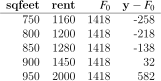
\includegraphics{figures/latex-1.svg}

(Many articles and Friedman's original paper call the values
pseudo-responses and use notation .)

The last column shows not only the direction but the magnitude of the
difference between where we are, \(F_0(X)\), and where we want to go,
\(y\). The red vectors in the following diagram are a visualization of
the residual vectors from our initial model to the rent target values.

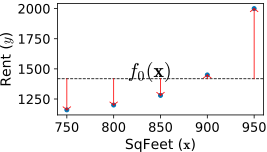
\includegraphics{figures/L2-loss_examples_3.svg}

Next, we train a weak model, \(\Delata_1\), to predict that residual
vector given \(x_i\) for all \(i\) observations. A perfect model,
\(\Delta_1\), would yield exactly \(y-F_0(X)\), meaning that we'd be
done after one step since \(F_1(X)\) would be
\(F_1(X) = F_0(X) + (y-F_0(X))\), or just \(y\). Because it imperfectly
captures that difference, \(F_1(X)\) is still not quite \(y\), so we
need to keep going for a few stages. Let's add learning rate, \(\eta\),
to our recurrence relation:

\[ F_m(X) = F_{m-1}(X) + \eta \Delta_m(X) \]

We'll discuss the learning rate below, but for now, please assume that
our learning rate is , so , , and so on. The following table summarizes
the intermediate values of the various key ``players'':

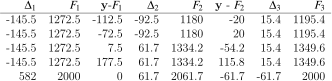
\includegraphics{figures/latex-65.svg}

It helps to keep in mind that we are always training on the residual
vector but get imperfect model . The best way to visualize the learning
of residual vectors by weak models, , is by looking at the residual
vectors and model predictions horizontally on the same scale Y-axis:

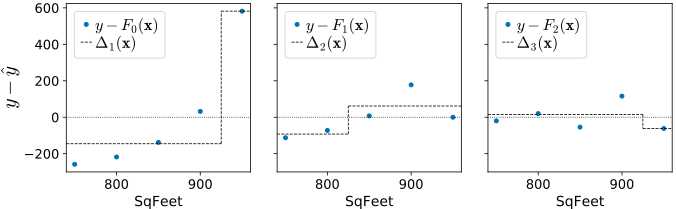
\includegraphics{figures/L2-loss_examples_4.svg}

The blue dots are the residual vector elements used to train weak
models, the dashed lines are the predictions made by , and the dotted
line is the origin at 0. Notice how the residual vector elements (blue
dots) get smaller as we add more weak models.

The predictions are step functions because we've used a regression tree
stump as our base weak model with split points 925, 825, and 925. Here
are the three stumps implementing our weak models:

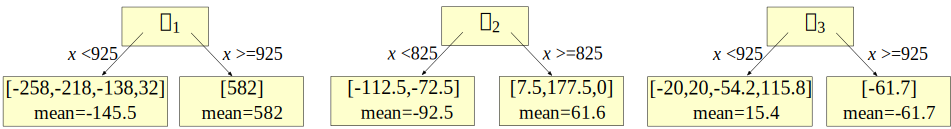
\includegraphics[width=1\linewidth]{figures/stubs-mse}

\textbf{Regression tree stumps}

A regression tree stump is a regression tree with a single root and two
children that splits on a single (feature) variable, which is what we
have here, at a single threshold. (If we had more than a single value in
our feature vectors, we'd have to build a taller tree that tested more
variables; to avoid overfitting, we don't want very tall trees,
however.) If a test feature value is less than the threshold, the model
yields the average of the training target samples in the left leaf. If
the test feature value is greater than or equal to the threshold, the
model yields the average of the training target examples in the right
leaf. The feature value split location is chosen to minimize the
variance of the target elements in each group. For example, imagine
single-valued features for 5 observations and target values . A good
place to split the feature values is between 1 and 4. That means
separating target values in the two leaves into very similar groups: and
.

The composite model sums together all of the weak models so let's
visualize the sum of the weak models:

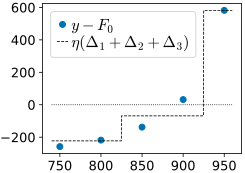
\includegraphics{figures/L2-loss_examples_5.svg}

If we add all of those weak models to the initial average model, we see
that the full composite model is a very good predictor of the actual
rent values:

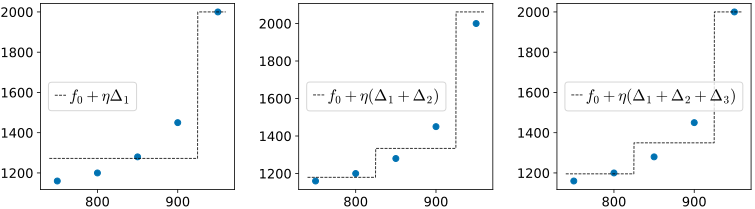
\includegraphics[width=1\linewidth]{figures/L2-loss_examples_6}

It's worth pointing out something subtle with the learning rate and the
notation used in the graphs: . That makes it look like the learning rate
could be applied all the way at the end as a global learning rate.
Mathematically, the formula is correct but it hides the fact that each
weak model, , is trained on and is a function of the learning rate: .
Friedman calls this incremental shrinkage.

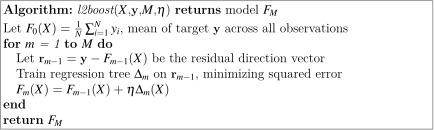
\includegraphics[width=1\linewidth]{figures/gbm-algorithm-l2-loss}

\section{\texorpdfstring{\href{https://quantdare.com/what-is-the-difference-between-bagging-and-boosting/}{What
is the difference between Bagging and
Boosting}}{What is the difference between Bagging and Boosting}}\label{what-is-the-difference-between-bagging-and-boosting}

Bagging and Boosting are both ensemble methods in Machine Learning, but
what's the key behind them?

Bagging and Boosting are similar in that they are both ensemble
techniques, where a set of weak learners are combined to create a strong
learner that obtains better performance than a single one. So, let's
start from the beginning:

What is an ensemble method? Ensemble is a Machine Learning concept in
which the idea is to train multiple models using the same learning
algorithm. The ensembles take part in a bigger group of methods, called
multiclassifiers, where a set of hundreds or thousands of learners with
a common objective are fused together to solve the problem.

The second group of multiclassifiers contain the hybrid methods. They
use a set of learners too, but they can be trained using different
learning techniques. Stacking is the most well-known. If you want to
learn more about Stacking, you can read my previous post, ``Dream team
combining classifiers``.

The main causes of error in learning are due to noise, bias and
variance. Ensemble helps to minimize these factors. These methods are
designed to improve the stability and the accuracy of Machine Learning
algorithms. Combinations of multiple classifiers decrease variance,
especially in the case of unstable classifiers, and may produce a more
reliable classification than a single classifier.

To use Bagging or Boosting you must select a base learner algorithm. For
example, if we choose a classification tree, Bagging and Boosting would
consist of a pool of trees as big as we want. Single Bagging and
Boosting 1 learner N learners From 1 to N Algorithm Comparison Versus

How do Bagging and Boosting get N learners? Bagging and Boosting get N
learners by generating additional data in the training stage. N new
training data sets are produced by random sampling with replacement from
the original set. By sampling with replacement some observations may be
repeated in each new training data set.

In the case of Bagging, any element has the same probability to appear
in a new data set. However, for Boosting the observations are weighted
and therefore some of them will take part in the new sets more often:
Single Bagging and Boosting Training set Multiple sets Random sampling
with replacement Over weighted data Algorithm Comparison VersusThese
multiple sets are used to train the same learner algorithm and therefore
different classifiers are produced.

Why are the data elements weighted? At this point, we begin to deal with
the main difference between the two methods. While the training stage is
parallel for Bagging (i.e., each model is built independently), Boosting
builds the new learner in a sequential way: Single Bagging and Boosting
Parallel Sequential Algorithm Comparison VersusIn Boosting algorithms
each classifier is trained on data, taking into account the previous
classifiers' success. After each training step, the weights are
redistributed. Misclassified data increases its weights to emphasise the
most difficult cases. In this way, subsequent learners will focus on
them during their training.

How does the classification stage work? To predict the class of new data
we only need to apply the N learners to the new observations. In Bagging
the result is obtained by averaging the responses of the N learners (or
majority vote). However, Boosting assigns a second set of weights, this
time for the N classifiers, in order to take a weighted average of their
estimates. Single Bagging and Boosting Single estimate Simple average
Weighted average Algorithm Comparison VersusIn the Boosting training
stage, the algorithm allocates weights to each resulting model. A
learner with good a classification result on the training data will be
assigned a higher weight than a poor one. So when evaluating a new
learner, Boosting needs to keep track of learners' errors, too. Let's
see the differences in the procedures: Single Bagging and Boosting
Training stage Train and keep Train and evaluate Update sample weights
Update learners weights Algorithm Comparison Versus

Some of the Boosting techniques include an extra-condition to keep or
discard a single learner. For example, in AdaBoost, the most renowned,
an error less than 50\% is required to maintain the model; otherwise,
the iteration is repeated until achieving a learner better than a random
guess.

The previous image shows the general process of a Boosting method, but
several alternatives exist with different ways to determine the weights
to use in the next training step and in the classification stage. Click
here if you like to go into detail: AdaBoost, LPBoost, XGBoost,
GradientBoost, BrownBoost.

Which is the best, Bagging or Boosting? There's not an outright winner;
it depends on the data, the simulation and the circumstances. Bagging
and Boosting decrease the variance of your single estimate as they
combine several estimates from different models. So the result may be a
model with higher stability.

If the problem is that the single model gets a very low performance,
Bagging will rarely get a better bias. However, Boosting could generate
a combined model with lower errors as it optimises the advantages and
reduces pitfalls of the single model.

By contrast, if the difficulty of the single model is over-fitting, then
Bagging is the best option. Boosting for its part doesn't help to avoid
over-fitting; in fact, this technique is faced with this problem itself.
For this reason, Bagging is effective more often than Boosting.

To sum up: Similarities

Differences

Both are ensemble methods to get N learners from 1 learner\ldots{}

\ldots{} but, while they are built independently for Bagging, Boosting
tries to add new models that do well where previous models fail.

Both generate several training data sets by random sampling\ldots{}

\ldots{} but only Boosting determines weights for the data to tip the
scales in favor of the most difficult cases.

Both make the final decision by averaging the N learners (or taking the
majority of them)\ldots{}

\ldots{} but it is an equally weighted average for Bagging and a
weighted average for Boosting, more weight to those with better
performance on training data.

Both are good at reducing variance and provide higher stability\ldots{}

\ldots{} but only Boosting tries to reduce bias. On the other hand,
Bagging may solve the over-fitting problem, while Boosting can increase
it.

\chapter{The bias-variance trade-off}\label{the-bias-variance-trade-off}

From \citep{pythonDataScienceHandBook}.

You can write citations, too. For example, we are using the
\textbf{bookdown} package \citep{R-bookdown} in this sample book, which
was built on top of R Markdown and \textbf{knitr} \citep{xie2015}.

\chapter{Literature}\label{literature}

Here is a review of existing methods.

\chapter{Methods}\label{methods}

We describe our methods in this chapter.

\chapter{Applications}\label{applications}

Some \emph{significant} applications are demonstrated in this chapter.

\section{Example one}\label{example-one}

\section{Example two}\label{example-two}

\chapter{Final Words}\label{final-words}

We have finished a nice book.

\section{R Markdown}\label{r-markdown}

This is an R Markdown document. Markdown is a simple formatting syntax
for authoring HTML, PDF, and MS Word documents. For more details on
using R Markdown see \url{http://rmarkdown.rstudio.com}.

When you click the \textbf{Knit} button a document will be generated
that includes both content as well as the output of any embedded R code
chunks within the document. You can embed an R code chunk like this:

\begin{Shaded}
\begin{Highlighting}[]
\KeywordTok{summary}\NormalTok{(cars)}
\end{Highlighting}
\end{Shaded}

\begin{verbatim}
##      speed           dist       
##  Min.   : 4.0   Min.   :  2.00  
##  1st Qu.:12.0   1st Qu.: 26.00  
##  Median :15.0   Median : 36.00  
##  Mean   :15.4   Mean   : 42.98  
##  3rd Qu.:19.0   3rd Qu.: 56.00  
##  Max.   :25.0   Max.   :120.00
\end{verbatim}

\section{Including Plots}\label{including-plots}

You can also embed plots, for example:

\includegraphics{myNotesBook_files/figure-latex/pressure-1.pdf}

Note that the \texttt{echo\ =\ FALSE} parameter was added to the code
chunk to prevent printing of the R code that generated the plot.

\bibliography{book.bib,packages.bib}


\end{document}
